\FILE{section-workflow.tex}

\subsubsection{Analytics Service Pipelines}

\paragraph{Motivation.}
In many cases a big data analysis is split up in multiple
subtasks. These subtasks may be reusable in other analytics
pipelines. Hence it is desirable to be able to specify and use them in
a coordinated fashion allowing reuse of the logic represented by the
analysis. Users must have a clear understanding on what the analysis
is doing and how it can be invoked and integrated.

\paragraph{Access Requirements.}
The analysis must include a clear and easy to understand specification
that encourages reuse and provides sufficient details about its
functionality, data dependency and performance. Analytics services may
have authentication, autorotation and access controls build in that
enable access buy users controlled by the service providers.



\begin{figure}[htb]
\centering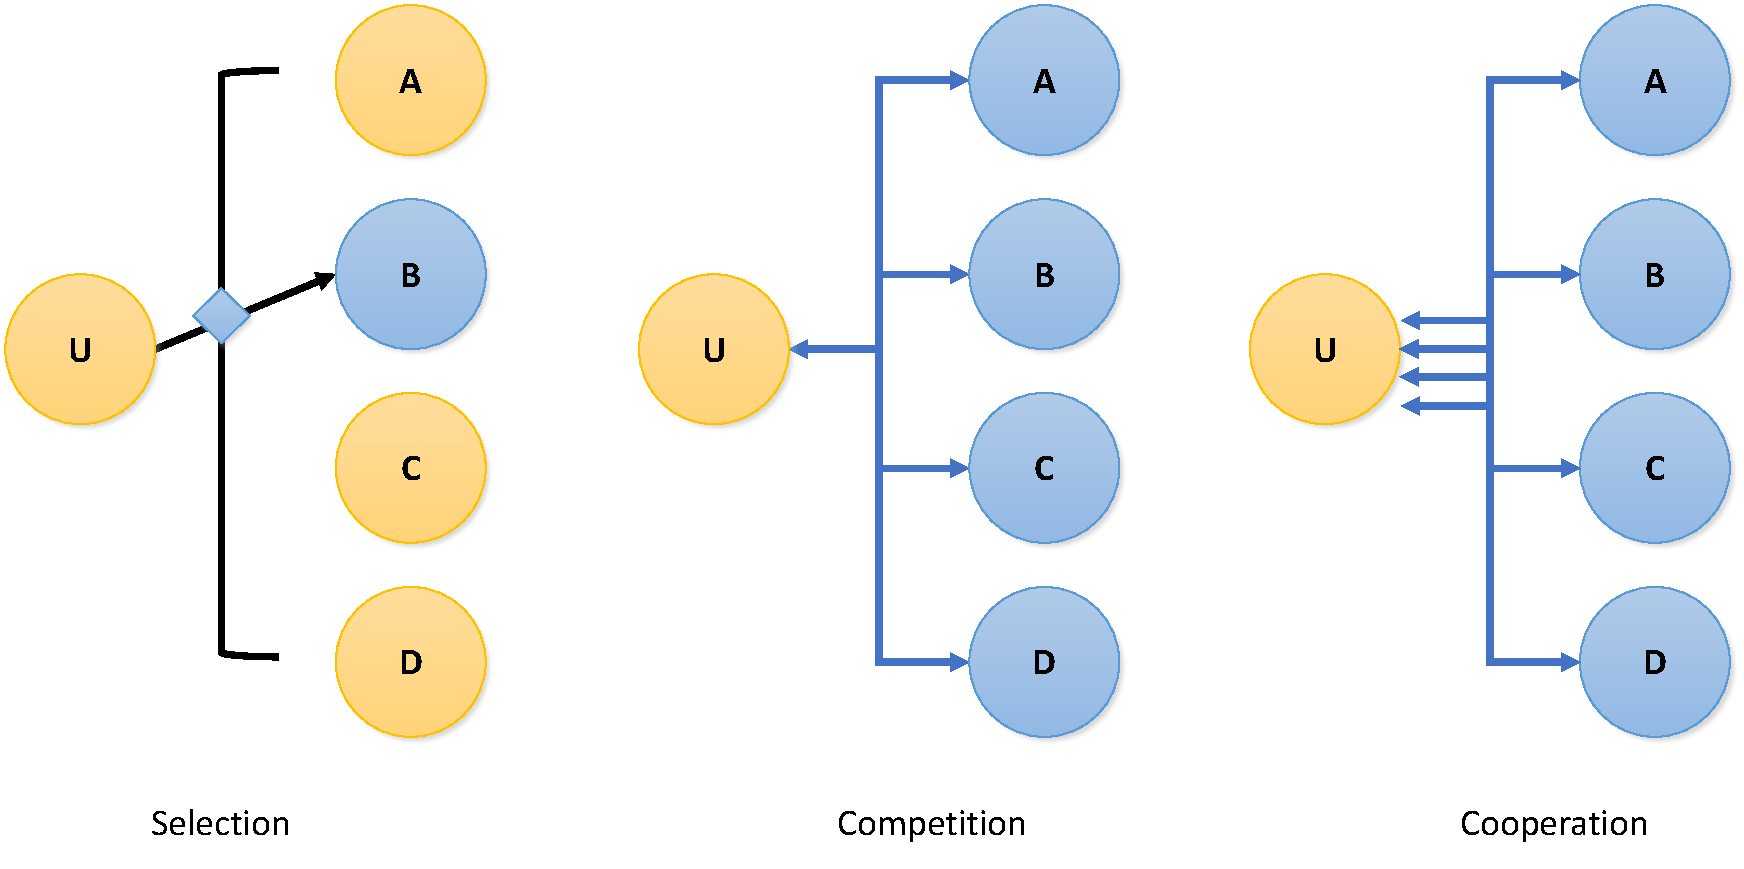
\includegraphics[width=1.0\columnwidth]{images/NIST-AI-services-workflow.pdf}
\label{fig:hvac-2}
\caption{Hybrid service integration.}
\end{figure}


\subsubsection{Workflow Controlled Computing}

High-performance computing (HPC) is for decades a very important tool for science. Scientific tasks can be leveraging the processing power of a supercomputer so they can run at previously unobtainable high speeds or utilize specialized hardware for acceleration that otherwise are not available to the user. HPC can be used for analytic programs that leverage machine learning applied to large data sets to, for example, predict future values or to model current states. For such high-complexity projects, 
there are often multiple complex programs that may be running repeatedly in either competition or cooperation. This may include resources in the same or different data centers. We developed 
a hybrid multi-cloud analytics service framework was created to manage heterogeneous and remote workflows, queues, and jobs. It can be used through an Python API, the command line, and a REST service. It is supported on multiple operating systems like macOS, Linux, and Windows 10 and 11. 
The workflow is specified via an easy to define YAML file.
Specifically, we have developed a library called Cloudmesh Controlled Computing (cloudmesh-cc) that adds workflow features to control the execution of jobs on remote compute resources, while at the same time leveraging capabilities provided by the local compute environments to directly interface with graphical visualizations better suited for the desktop. The goal is to provide numerous workflows that in cooperation enhances the experience of the analytics tasks. This includes a REST service and command line tools to interact with it.


\begin{figure}[htb]
\centering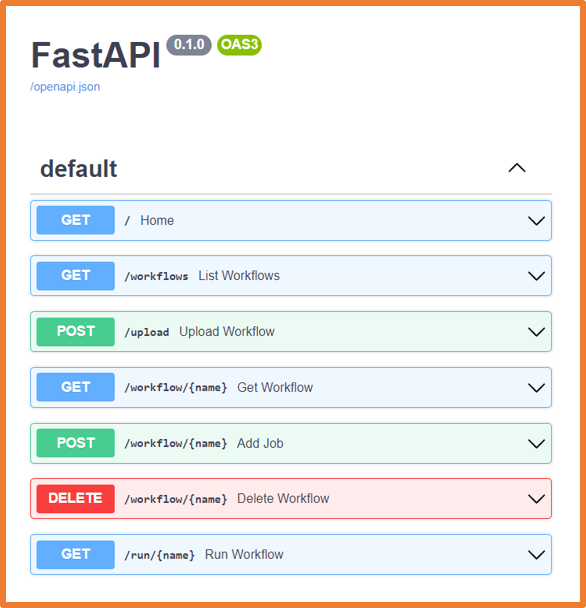
\includegraphics[width=0.7\columnwidth]{images/fastapi-service.png}
\caption{Fast API Workflow Service.}
\label{fig:fastapi-cc-arch}
\end{figure}

\begin{figure}[htb]
    \centering
    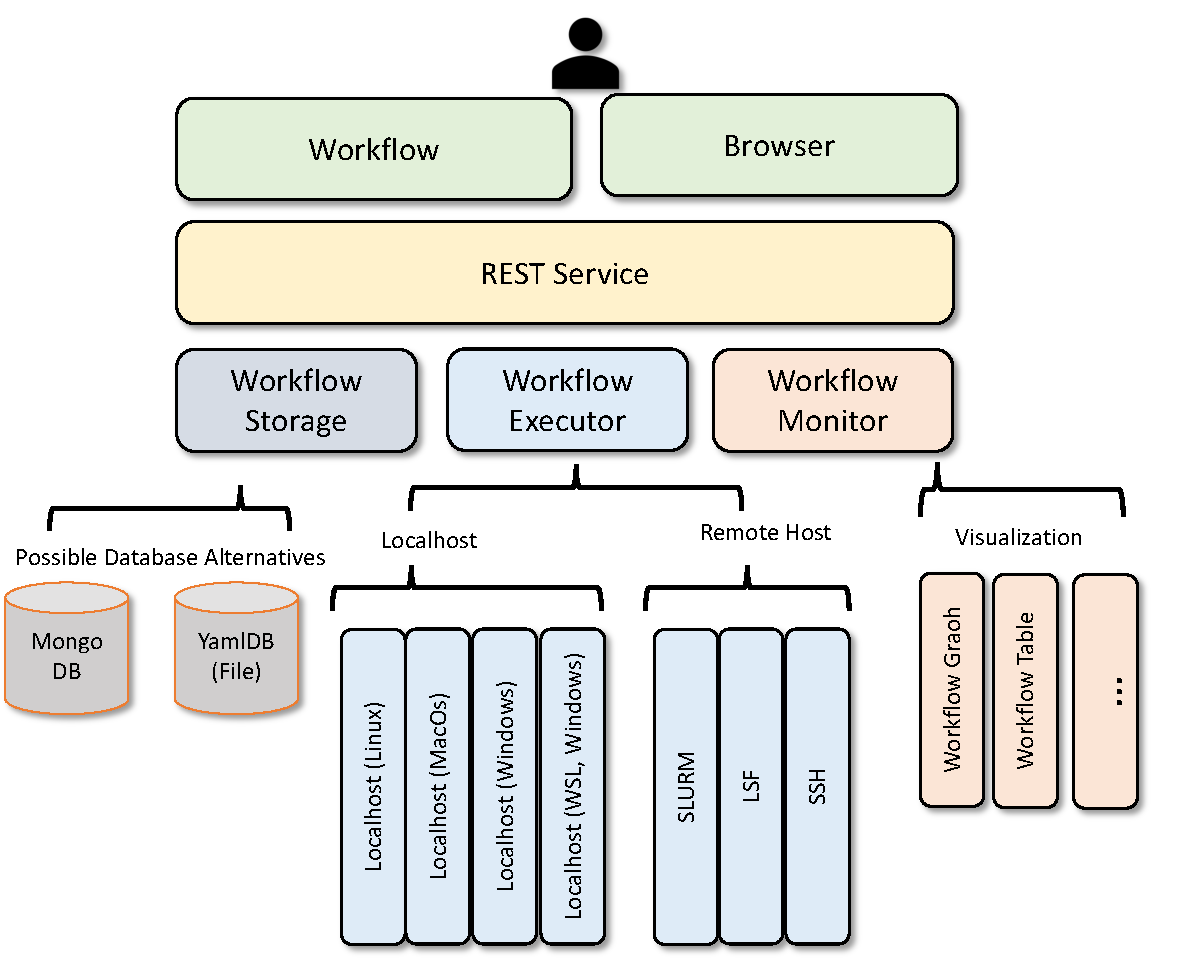
\includegraphics[width=1.0\columnwidth]{images/cc.pdf}
    \caption{Architecture Workflow Service.}\label{fig:cc-2}
\end{figure}

\begin{figure}[htb]
    \centering
    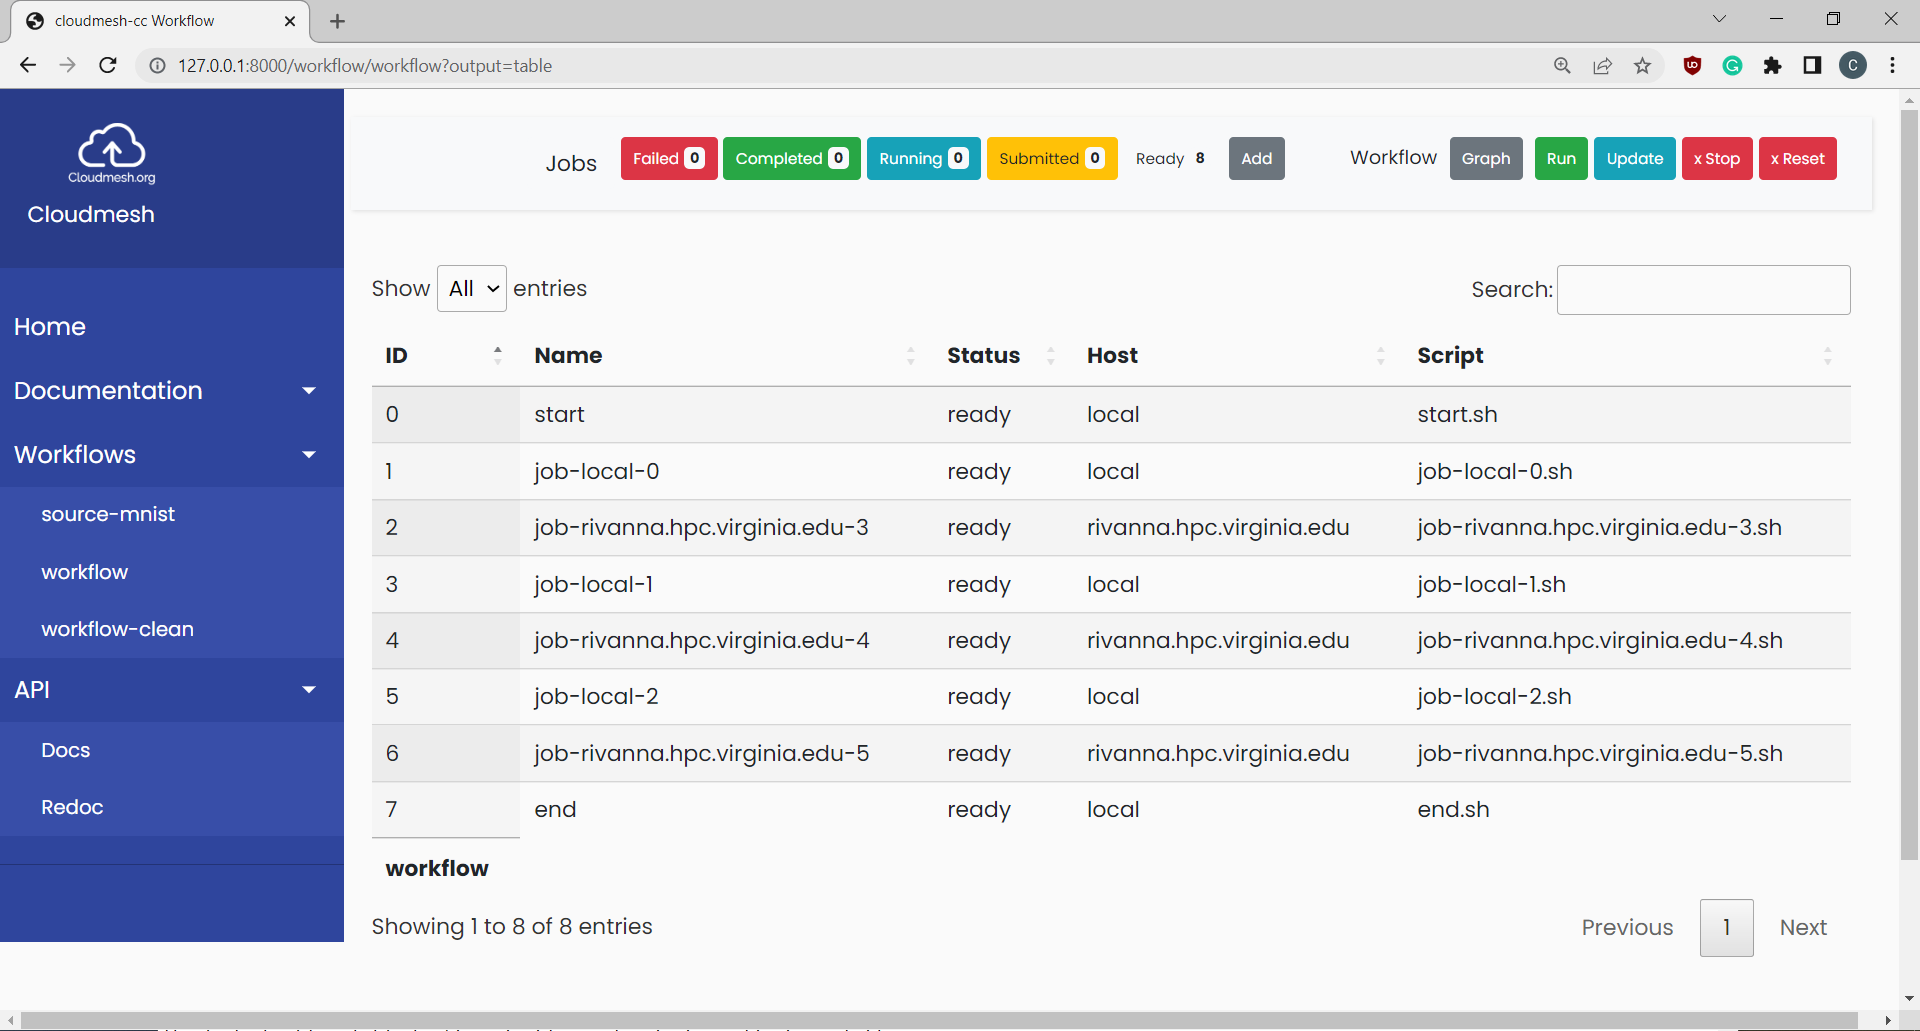
\includegraphics[width=1.0\columnwidth]{images/cc-1.png}
    \caption{Workflow user interface.}\label{fig:cc-3}
\end{figure}

We have tested the framework while running various MNIST application examples, including include Multilayer Perceptron, LSTM (Long short-term memory), Auto-Encoder, Convolutional, and Recurrent Neural Networks, Distributed Training, and PyTorch training. 
A much lager application using earthquake prediction has also been used.

Figure \ref{fig:fastapi-cc-arch} shows the REST specification and Figure \ref{fig:cc-2} shows the architecture. A user interface of the running application is shown in Figure \ref{fig:cc-3}.

% \subsubsection{Federated Analytics Service Catalogue}
% \subsubsection{Catalogue Attributes}
% \subsubsection{Federated analytics service Registries}
% \subsubsection{Registry Attributes}

% \subsection{Resource Accessibility}
% \subsubsection{Resource Management}
% \subsubsection{Security}

